\chapter{Related Work}
\label{chapter:Related_Work}

\begin{figure}[h!]
  \centering
    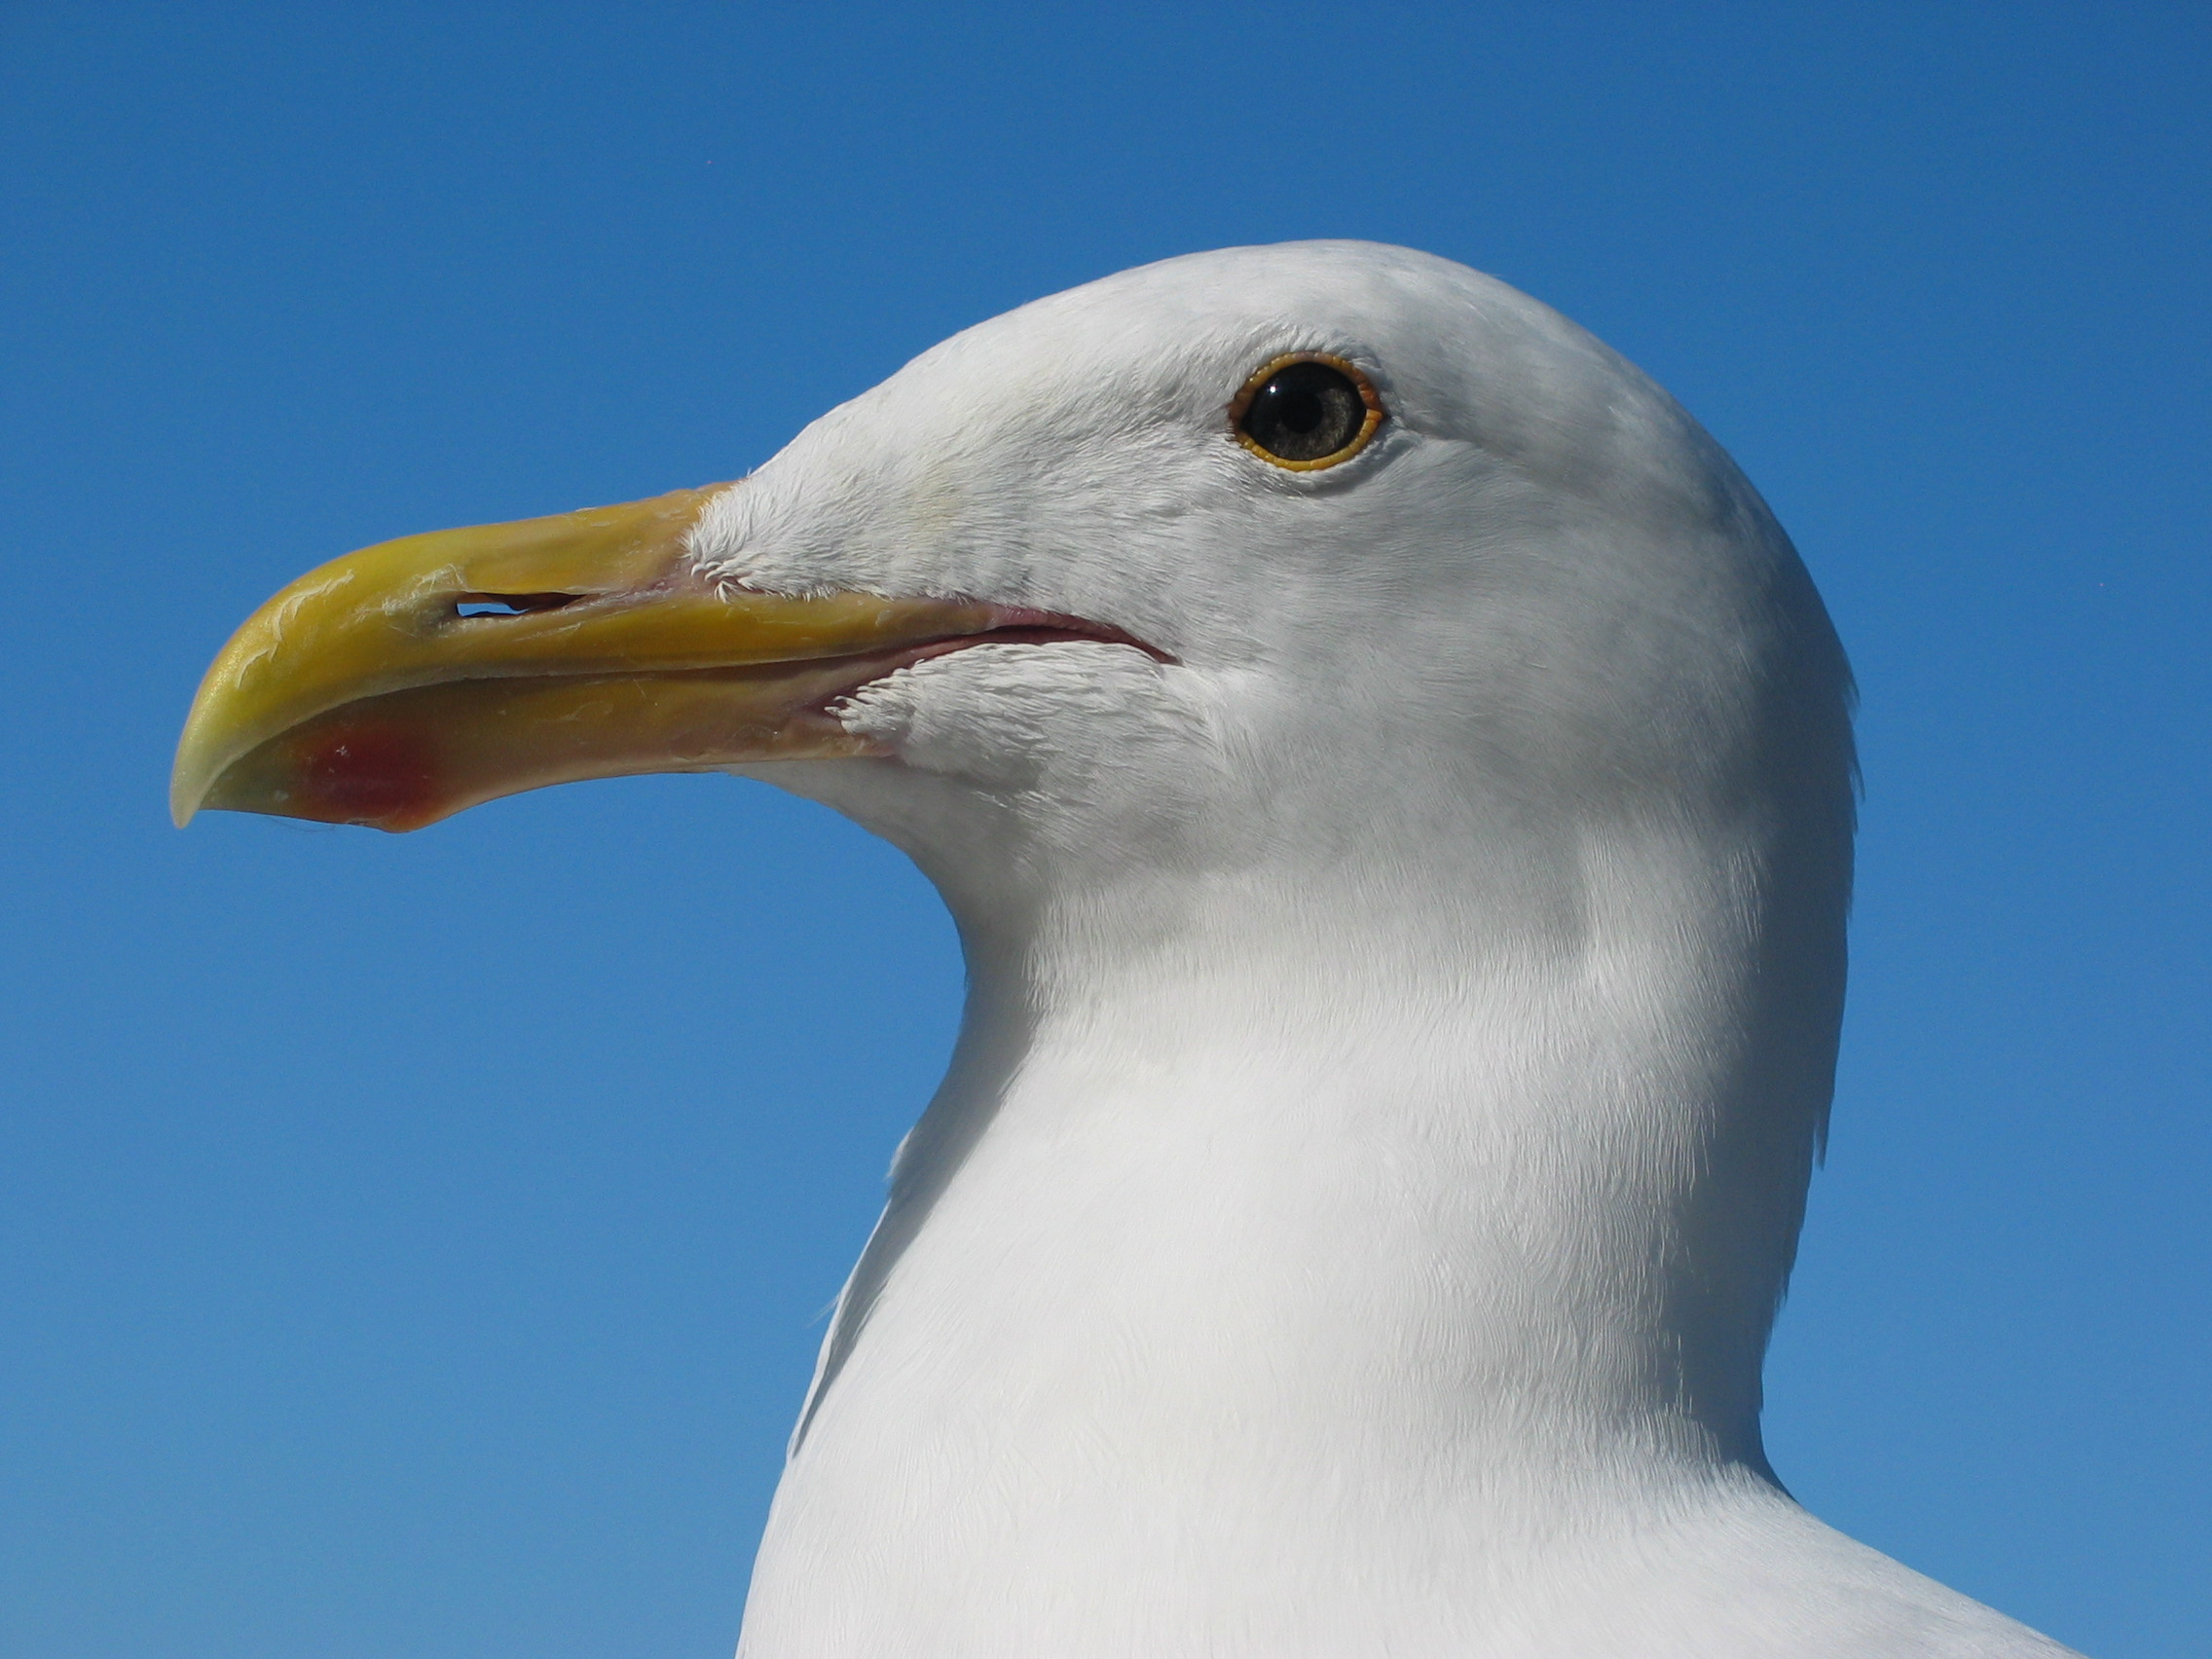
\includegraphics[width=0.8\textwidth]{chapters/images/gull}
  \caption{A picture of a gull.}
\end{figure}

\section{3D geometry}

Yes  - do coordinate systems, transformations, notation
Brief description of SE(3) and SO(3)

\section{Camera Models}

In order to utilise a camera as a sensor, a mapping between image coordinates and world
coordinates needs to be derived.  This allows observations of the camera to be transformed into
meaningful measurements.  To achieve this mapping a sensor model of the camera is required. This
section will cover all the different types of cameras used in this work and corresponding camera
models for each. 

\subsection{Pinhole Camera Model}
\label{subsec:pinhole_cam}

%TODO: references

The pinhole camera model is the most basic and common of camera models used in computer vision.  It
describes the mathematical relationship between the coordinates of a 3D point in the world and its
projection onto an image plane.  This model assumes the aperture of the camera to be an ideal
pinhole. It does not consider lenses used to focus light which in reality result in lense
distortion.  It does also not take into account sensor quantization apparent in using a modern
digital CCD sensor. Nevertheless it still provides a sufficient model of camera projection for this
work, and practical considerations such as image size, resolution and lense distortion can be
compensated for.

When using the pinhole camera model, the camera is assumed to be a sealed box with a pinhole
aperture on one side, and the image plane, or image sensor on the other side.  Having a small
aperture blocks most of the light rays from objects in the world and allows a focused and inverted
image of the world to be recorded. In this case the focal point is the aperture and the focal length
is the distance from the aperture to the sensor. fig. whatever. For all intensive purposes,
this model can be redrawn as in fig. whatever whatever. The image plane is inverted and shown
reflected in front the of the camera.  As long as the focal length can be determined, it is then
trivial to calculate coordinates on the sensor for a given ray or world coordinate using simple
geometry. Sensor coordinates can then be converted to image coordinates given the physical size
of the CCD and its resolution.  

Take note the principle point is often not in the sensor of the image, and therefore the
coordinates of this point on the sensor needs to be determined.  In addition the focal length
varies from camera to camera and therefore both of these values need to be determined by performing
an intrinsic calibration. For the calibration, the focal length may be expressed in pixel units,
which means the conversion from metric sensor coordinates ( m) to pixel coordinates (u,v) is
also performed in one step.

%http://www.jordicenzano.name/projects/2D-to-3D-Paradigm-overview/camera-model
%use this for picture motivation

\begin{figure}[h!]
  \centering
    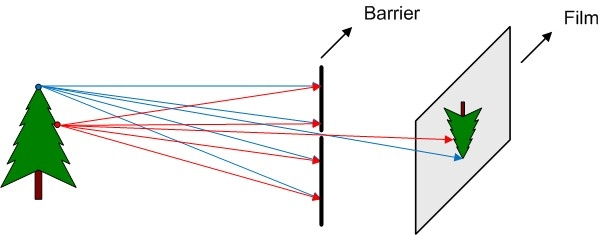
\includegraphics[width=0.5\textwidth]{chapters/images/cam_model_fig2}
  \caption{Pinhole camera model}
\end{figure}

\begin{figure}[h!]
  \centering
    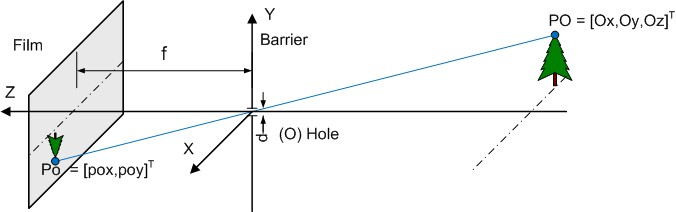
\includegraphics[width=0.9\textwidth]{chapters/images/cam_model_fig41} \\
    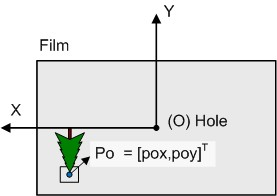
\includegraphics[width=0.3\textwidth]{chapters/images/cam_model_fig42} \\
    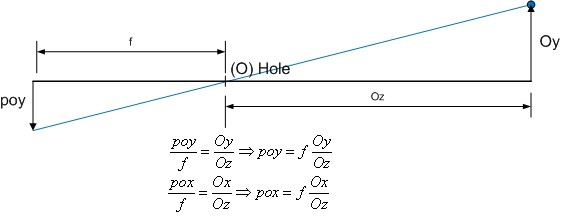
\includegraphics[width=0.9\textwidth]{chapters/images/cam_model_fig43} 
  \caption{Pinhole camera model with image plane shown inverted in front of the focal point}
\end{figure}

%%TODO: I stole these pictures.  I want to redraw them myself

\subsection{Lense Distortion}

%TODO: references

The problem with using a pinhole camera in practice is that it does not allow enough light to into
the camera, requiring longer exposure time and therefore blurring in the presence of movement. 
Therefore a double convex lense is used to focus more light rays onto the sensor and allowing a
sharper image.  Such as setup can be seen in fig. xyz.  The pinhole camera model may still be used,
however now lense distortion needs to be accounted for.  Lense distortion causes lines to be
curved, as in fig x.  It is also possible during the intrinsic calibration to simultaneously
determine distortion coefficients which allow the image to be reshaped such that all straight lines
appear straight.

\begin{figure}[h!]
  \centering
    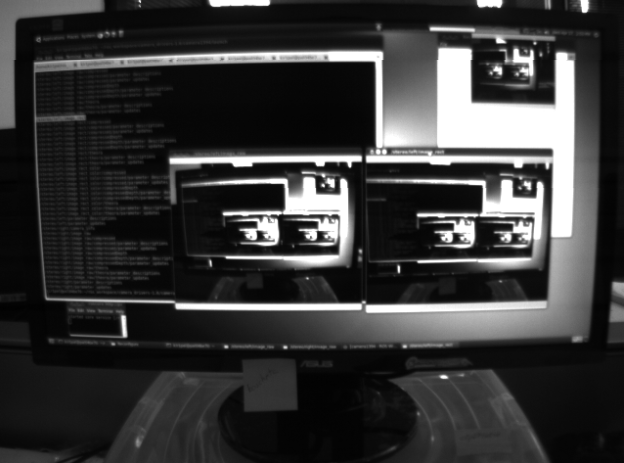
\includegraphics[width=0.49\textwidth]{chapters/images/distorted}
    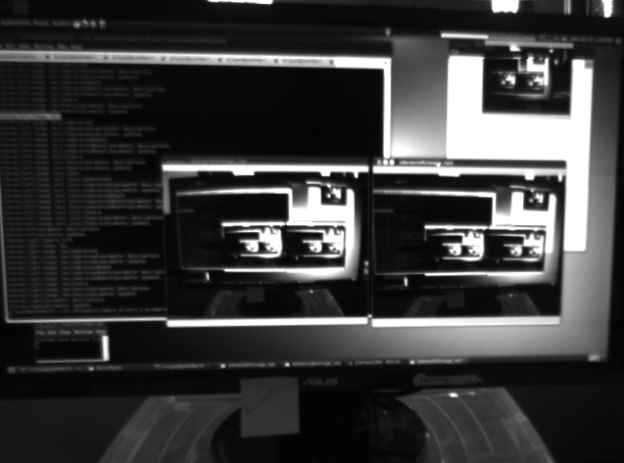
\includegraphics[width=0.49\textwidth]{chapters/images/undistorted}
  \caption{Left: An image with lense distortion.  Right: The same image with lense distortion
compensated for}
\end{figure}

\subsection{Homogeneous coordinates}

%%TODO: homogeneous coordinates

\begin{equation}
 \begin{pmatrix}
  u \\
  v \\
  1 
 \end{pmatrix} =
 \begin{pmatrix}
  f_x & 0 & c_x \\
  0 & f_y & c_y \\
  0 & 0   & 1 
 \end{pmatrix}
 \begin{pmatrix}
  X \\ Y \\ Z
 \end{pmatrix}
\end{equation}


\subsection{Stereo Camera}

\subsection{Omni-directional Camera}

% ask matthias for literature

\subsection{Flir}
Leave this to last.  Flir may (probably) get left out

\section{Computer Vision Basics}

\subsection{Feature point detection and extraction}
\label{subsec:features}

Outline what is feature point detection, description and matching, why we need
it.  Mention SIFT
and SURF and cite them.  Mention that we used a GPU implemtation of SIFT, cite
the ETH paper. 
Mention a bunch of other descriptors, cite them as well.

\subsection{RANSAC}
\label{subsec:RANSAC}

explain this cos its easy and fun.  Cite a paper

\subsection{Geometry estimation}

\subsubsection{5 point algorithm}
\label{subsec:5point}
ask for matthias for relavent literature

\subsubsection{Point triangulation}

ask for matthias for relavent literature

\subsubsection{Stereo pose estimation}
\label{subsec:horn}

Umeyama (PCL) \newline 
Horn (UVM)


\section{Place Recognition}

Bag of words

\section{Visual SLAM}

%Cover this in abstract terms.  Talk about the theory, not implemtation.  Mention
%PTAM and cite it.
%No g2o here.

Simulataneous Localization and Mapping (SLAM) is the technique of building a map of a previously
unexplored area whilst simultaneously determining a position (localizing) within that map.  The
traditional approach for SLAM can be split into 4 steps.
\begin{enumerate} \itemsep1pt \parskip0pt \parsep0pt
 \item Feature extraction
 \item Data association
 \item Pose estimation
 \item Global Optimization
\end{enumerate}

%TODO: cite kalman filter
Feature extraction involves finding unique features within the sensor data, also known as
landmarks, which can be later in future sensor measurements.  Data association is the process of
matching these landmarks over multiple sensor readings, in essence tracking them.  Pose estimation
involves using the information of how multiple landmarks moved over time with respect to the
robot/sensor in order to determine how the robot moved with respect to those landmarks.  Finally,
having determined a map of landmarks, and a pose with respect to those landmarks, a global
optimization, or bundle adjustment, over all landmarks and robot poses may be performed in order to
produce a globally consistent map and trajectory.  In the past this has commonly been done by using
a kalman filter (cite) and by adding all landmarks to the system state.  In more recent times graph
optimization approaches have become popular as they scale much better to larger maps.

SLAM has taken many forms depending on sensors available. Visual SLAM denotes performing SLAM using
some kind of camera.  In recent times, a plethora of visual SLAM algorithms for monocular cameras
(cite andrew davidson slam, ptam, something else), stereo cameras (more citations) and RGBD cameras
(rgbdslam, kinfu, kintinuous) have been developed.  A keyframe SLAM system similar in concept to the
PTAM approach has been utilised as the basis for this work.  The basic operation for this style of
SLAM will be outlined here.

\subsection{Basic VSLAM pipeline}

The following is a description of a basic pipeline for visual SLAM.  Whilst the SLAM system that
this work is based on is somewhat more complex, this shows how all the above algorithms may be used
together to form a complete SLAM pipeline.  The utilised SLAM system will be discussed in section
\ref{chapter:ScaViSLAM}

The feature extraction in Visual SLAM involves using image feature detectors/ descriptors as
outlined in section \ref{subsec:features}.  These features may then be referred to as
landmarks. For a single observation of a landmark from one frame of a single camera, one can
determine a 3D ray from the current camera pose by making use of the camera model as outlined in
section \ref{subsec:pinhole_cam}.  Multiple observations from multiple frames allows for multiple
rays to intersect at this landmark, thus a 3D position of the landmark may be estimated using
triangulation. In the case of a stereo camera, the 3D estimate more or less comes for free, as
landmarks may be triangulated from left and right camera frame.

The data association stage is performed by doing feature matching across different camera frames.
Pose estimation is commonly achieved by utilising the RANSAC algorithm (\ref{subsec:RANSAC}) 
This can be coupled with the 5 point algorithm (\ref{subsec:5point}) in the case of monocular SLAM
(2D-2D correspondances), or with Umeyama/Horn (\ref{subsec:horn}) for stereo or RGBD, (3D-3D
correspondances). The model in this case is the 6 DoF transform between frames. The error is
calculated by projecting landmarks from one frame to the next by applying the transformation to each
of them. The error is then the sum of the distances between points of one frame, and the
corresponding points transformed to that same frame. \ref{eq:ransac_error}

\begin{figure}
 \centering
 \begin{math}
  e = \sum\limits_{p_i} p^a_i - _aT^b \cdot p^b_i
 \end{math}
 \caption{RANSAC error function.  this formula sucks needs formatting}
 \label{eq:ransac_error}
\end{figure}


Bundle adjustment over all landmarks and camera poses is commonly achieved with a graph
optimization. This will be expanded on in sec \ref{subsec:graph_slam}

\subsection{Keyframe SLAM}

The main idea behind keyframe SLAM is to divide the tasks of localization and mapping, and have
them run in parallel is separate threads.  The mapping thread defines a keyframe to track against. 
This amounts to a global pose of the keyframe, as well as a number of landmarks visible from that
keyframe recorded relative to that keyframe pose.  The localization thread localizes the camera
with respect to that keyframe.  If the camera moves or rotates a significant distance away from
the active keyframe, a new keyframe will be created with a known transformation to the previous
keyframe.

The intent is to have a fast localization thread that runs in realtime providing an accurate pose
estimation with respect to the keyframe.  The mapping thread that deals with the keyframe runs at a
much lower framerate, and handles changing the keyframe, global optimization(?), something else. 
The overall outcome is a system that provides an accurate pose in global coordinates with a fast
update rate, as well as a globally consistent map.

\subsection{Graph SLAM}
\label{subsec:graph_slam}
